\iffalse
\documentclass[12pt]{article}
\usepackage{graphicx}
\usepackage{amsmath}
\usepackage{mathtools}
\usepackage{gensymb}

\newcommand{\mydet}[1]{\ensuremath{\begin{vmatrix}#1\end{vmatrix}}}
\providecommand{\brak}[1]{\ensuremath{\left(#1\right)}}
\providecommand{\norm}[1]{\left\lVert#1\right\rVert}
\newcommand{\solution}{\noindent \textbf{Solution: }}
\newcommand{\myvec}[1]{\ensuremath{\begin{pmatrix}#1\end{pmatrix}}}
\let\vec\mathbf
\def\inputGnumericTable{}
\usepackage{color}                                            %%
    \usepackage{array}                                            %%
    \usepackage{longtable}                                        %%
    \usepackage{calc}                                             %%
    \usepackage{multirow}                                         %%
    \usepackage{hhline}                                           %%
    \usepackage{ifthen}
\usepackage{array}
\usepackage{amsmath}   % for having text in math mode
\usepackage{listings}
\lstset{
language=tex,
frame=single, 
breaklines=true
}
\begin{document}
\begin{center}
\textbf\large{CLASS-9\\CHAPTER-10 \\ CIRCLES}

\end{center}
\section*{Excercise 10.5}

Q1. section*{\large Solution}
\fi
\begin{figure}[H]
\centering
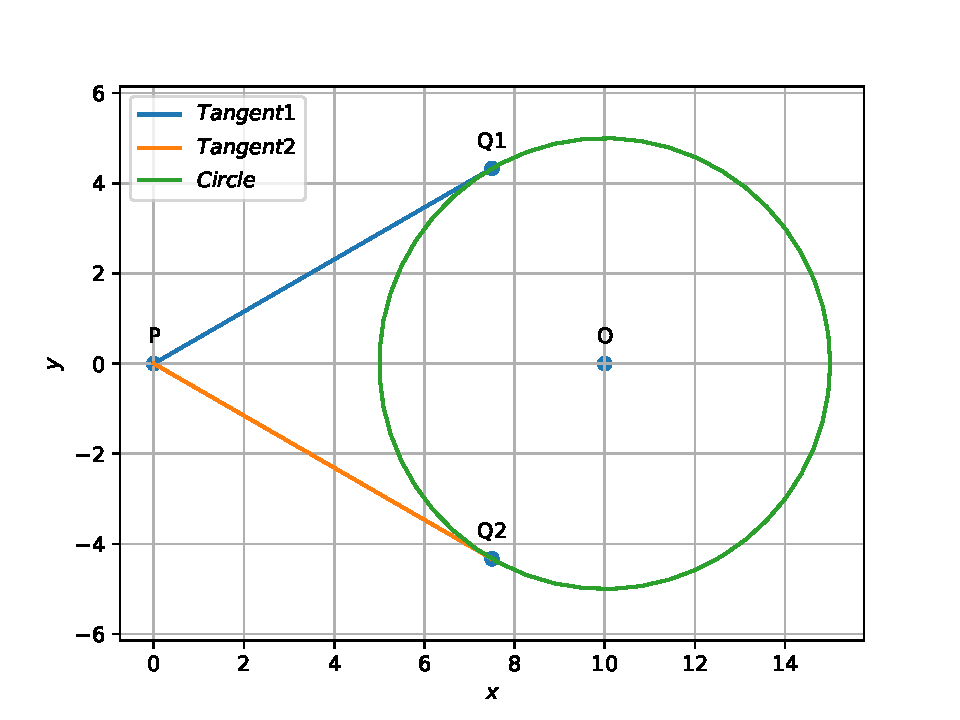
\includegraphics[width=0.75\columnwidth]{chapters/9/10/5/1/figs/circle1.pdf}
\caption{}
\label{fig:chapters/9/10/5/1/Fig1}
\end{figure}
%
\begin{table}[H]
	\centering
	%\subimport{../chapters/9/10/5/1/tables/}{table1.tex}
     \begin{tabular}{|p{3cm}|p{3cm}|p{3cm}|}
\hline                                        
\textbf{Symbol} & \textbf{Values} & \textbf{Description}\\                                          
\hline                                 
$\theta$ & 30$\degree{}$   & $\angle{BAD} = \angle{BAC}$ \\           
\hline                                    
a &  9 & $AB$ \\     
\hline                      
c & 5 & $AC$ \\
\hline                                     
		$\vec{e}_1$ & $\myvec{
			1\\
			0\\
			}$ & basis vector\\ 
\hline
\end{tabular}

%	\caption{}
	\label{table:chapters/9/10/5/1/table1}
	\end{table}
The input parameters are available in Table
	\ref{table:chapters/9/10/5/1/table1} yielding
\begin{align}
	\vec{C} =\vec{e}_1= \myvec{1\\0},\,
	\vec{A} = \myvec{\cos(\alpha+\beta)\\\sin(\alpha+\beta)},\,
	\vec{D} = \myvec{\cos\gamma\\\sin\gamma}.
\end{align}
Since
\begin{align}
	 \vec{A-D}& = \myvec{\cos(\alpha+\beta) - \cos\gamma\\\sin(\alpha+\beta) - \sin\gamma},
	 \vec{C-D} &= \myvec{1 - \cos\gamma\\-\sin\gamma},
	 \norm{\vec{A-D}}\norm{\vec{C-D}}& = 4 \sin\frac{\alpha+\gamma}2\sin\frac{\beta+\gamma}2,
	 \\
	\cos(\angle ADC) &= \frac{\vec{(A-D)^\top(C-D)}}{\norm{\vec{A-D}}\norm{\vec{C-D}}},
	\label{eq:2}
	\\
	&= 4\sin\frac{\alpha+\gamma}2\sin\frac{\beta+\gamma}2\cos\frac{\alpha+\beta}2
 = \cos\frac{\alpha+\beta}{2}
	\label{eq:7}
\end{align}
Substituting $\alpha$ and $\beta$ in \eqref{eq:7}
\begin{align}
\angle ADC = \frac{\alpha+\beta}{2}=\frac{(30\degree + 60\degree )}{2}=45\degree
\end{align}
See Fig. 
\ref{fig:chapters/9/10/5/1/Fig1}.


